\chapter{Entwurfsmuster}

\section{Entwurfsmuster: Observer-Pattern}

\autoref{fig:observer} zeigt das Observer-Pattern, wobei ein \textit{GameEndObserver} von einem \textit{GameEndObservable} benachrichtigt 
wird, wenn das Spielende erreicht ist und mit einem \textit{GameResult} abgeschlossen wird. Das UML zeigt das 
konkrete GameEndObservable \textit{GameState}, welches seine GameEndObservers updated, wenn das GameResult über einen 
Setter geändert wird. Der konkrete GameEndObserver \textit{GameEndReporter} aus der Plugin-Schicht gibt dann 
das Spielergebnis an den User aus. Hierfür wird der GameEndReporter in der \textit{main}-Methode erzeugt und über 
DI an die höhere Schicht weitergegeben. \\ 
Das Observer-Pattern ist hier sehr sinnvoll, da das Spielende ein Zustand ist, 
der über viele verschiedene Wege und User-Befehle erreicht werden kann, wie zum Beispiel das Ziehen der letzten 
Karte, ohne dass noch eine Aktion möglich ist, oder der Spieler mit dem letzten möglichen Endeavor nicht erfolgreich ist usw. 
Daher ist es sinnvoll dies über ein Event abzuwickeln, damit nicht viele verschiedene Commands separat auf Spielende checken müssen, 
was auch gegen das SRP gehen würde. Außerdem erlaubt es eine sehr flexible Erweiterbarkeit, wenn zum Beispiel ein 
Highscore-Mechanismus eingebaut werden soll, der am Spielende die benötigten Züge abspeichert.      

\begin{figure}[H]
	\centering
	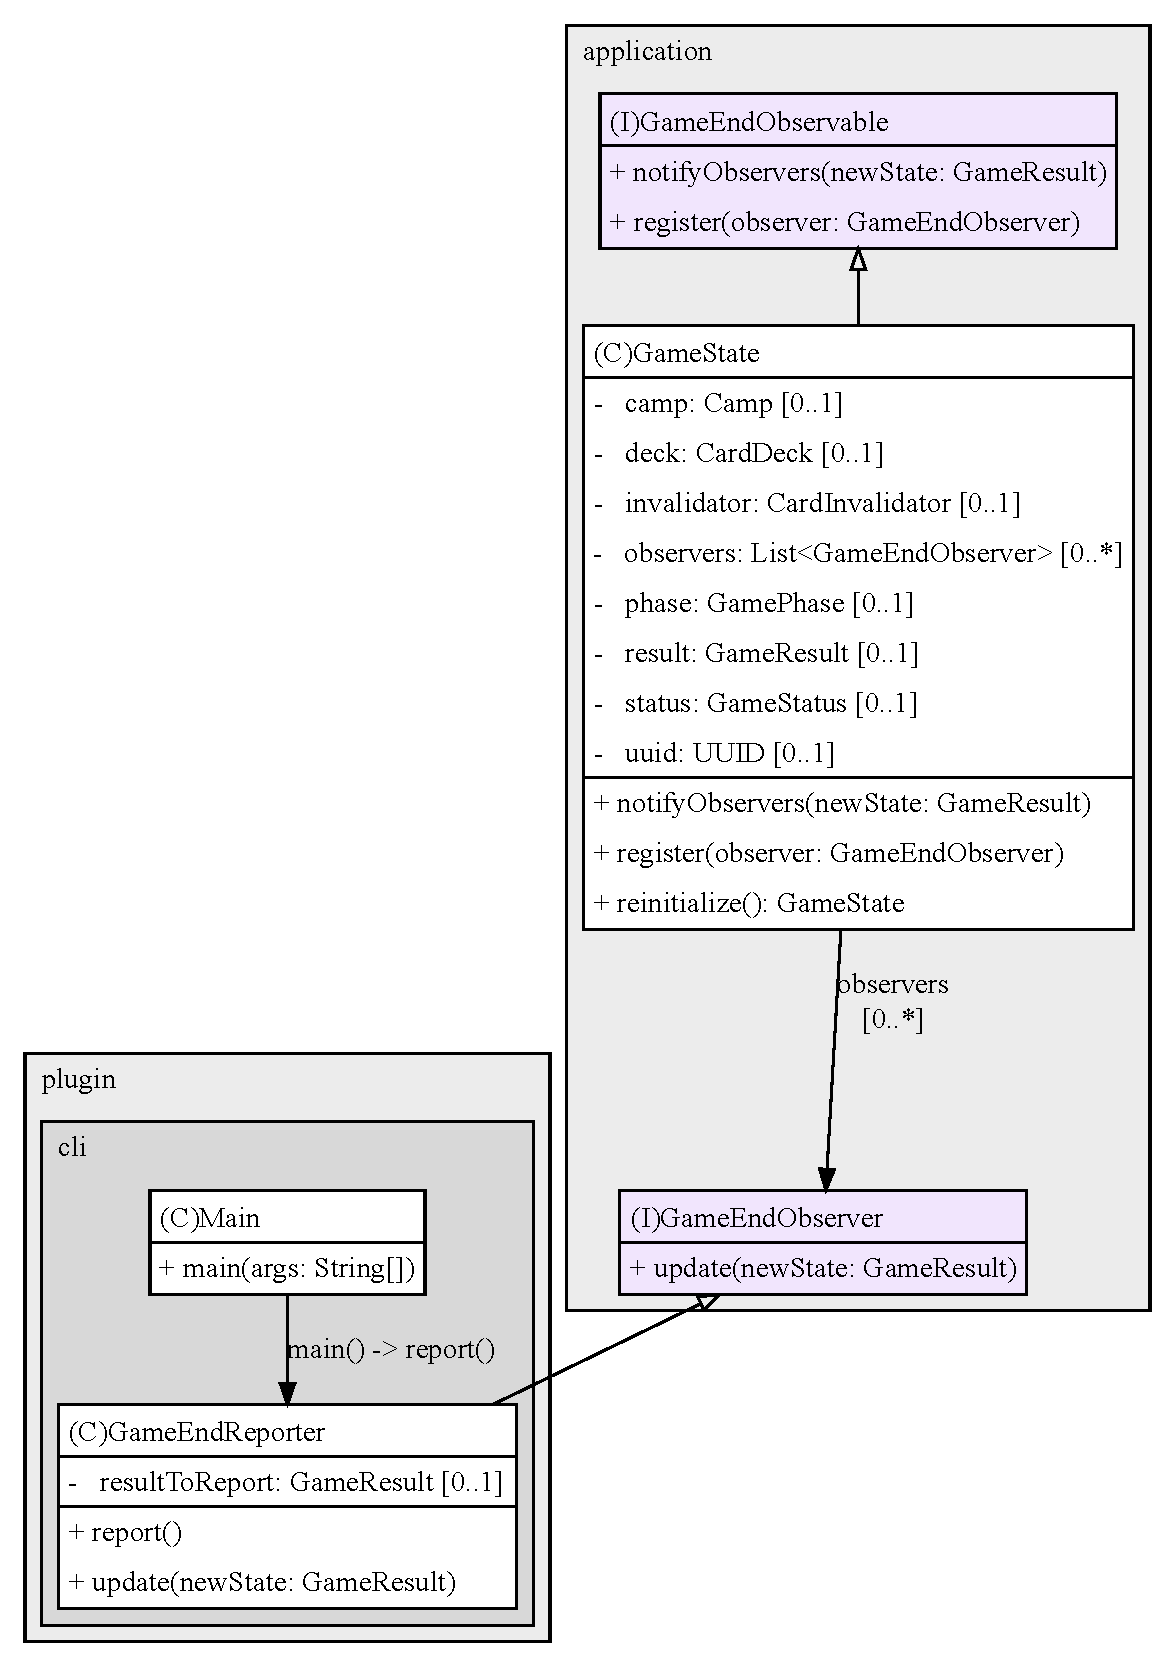
\includegraphics[width=0.6\textwidth]{Bilder/GameEndObserver_structure.pdf} 
	\caption{UML-Diagramm des Observer-Patterns zwischen \textit{GameState} und \textit{GameEndReporter}.}
	\label{fig:observer}
\end{figure} 

\section{Entwurfsmuster: Strategie}

\autoref{fig:strategy} zeigt das Stragie-Entwurfsmuster für die Logik der unterschiedlichen Endeavor-Möglichkeiten. 
Hierzu hält der Anwender \textit{RollHandler} eine Referenz auf die Strategie \textit{Rescue}, für die die 
Methode \textit{endeavor} implementiert werden muss. Die konkreten Strategien \textit{GuaranteedRescue} und \textit{PossibleRescue}
implementieren das Interface und können so flexibel von dem Anwender RollHandler verwendet werden. \\ 
Das Pattern ergibt hier sehr viel Sinn, da der RollHandler die konkrete Berechnung, ob das Endeavor geglückt ist oder nicht, 
nicht selbst durchführen muss, bzw. davon nichts wissen muss. Das unterstützt sehr stark das OCP, SRP und geringe Kopplung. 
Sollte eine weitere Form der Rescue eingeführt werden und möglich werden, ist das Programm so sehr flexibel und einfach 
erweiterbar.  

\begin{figure}[H]
	\centering
	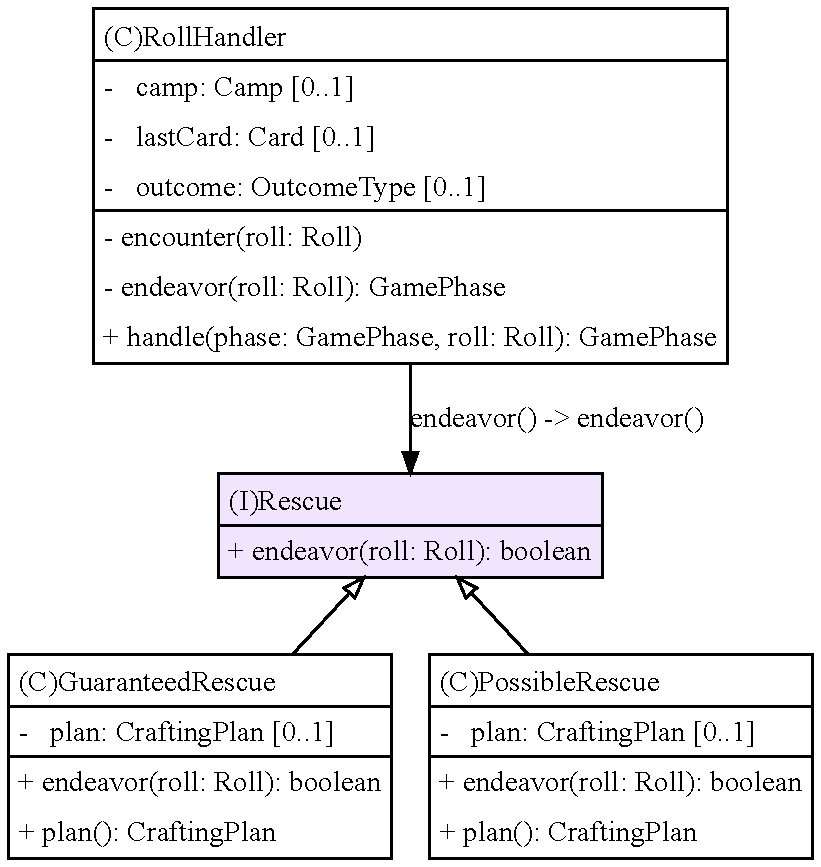
\includegraphics[width=0.5\textwidth]{Bilder/Rescue_structure.pdf} 
    \caption{UML-Diagramm (gekürzt) des Strategie-Pattern der \textit{Rescue-Endeavor}-Logik. Zur besseren Übersichtlichkeit 
    wurden überflüssige Klassen ausgelassen.}
	\label{fig:strategy}
\end{figure} 